% floorplan.tex
% Scaled site/floor plan, 1/4" = 1'-0", drawn on an 8.5in x 11in sheet.
% Every TikZ coordinate below is in real page inches, so the drawing
% reproduces the hand sketch's measurements exactly as taken with a ruler.
\documentclass[letterpaper]{article}
\usepackage[paperwidth=8.5in,paperheight=11in,margin=0in]{geometry}
\usepackage{tikz}
\usetikzlibrary{arrows.meta}
\pagestyle{empty}

\begin{document}
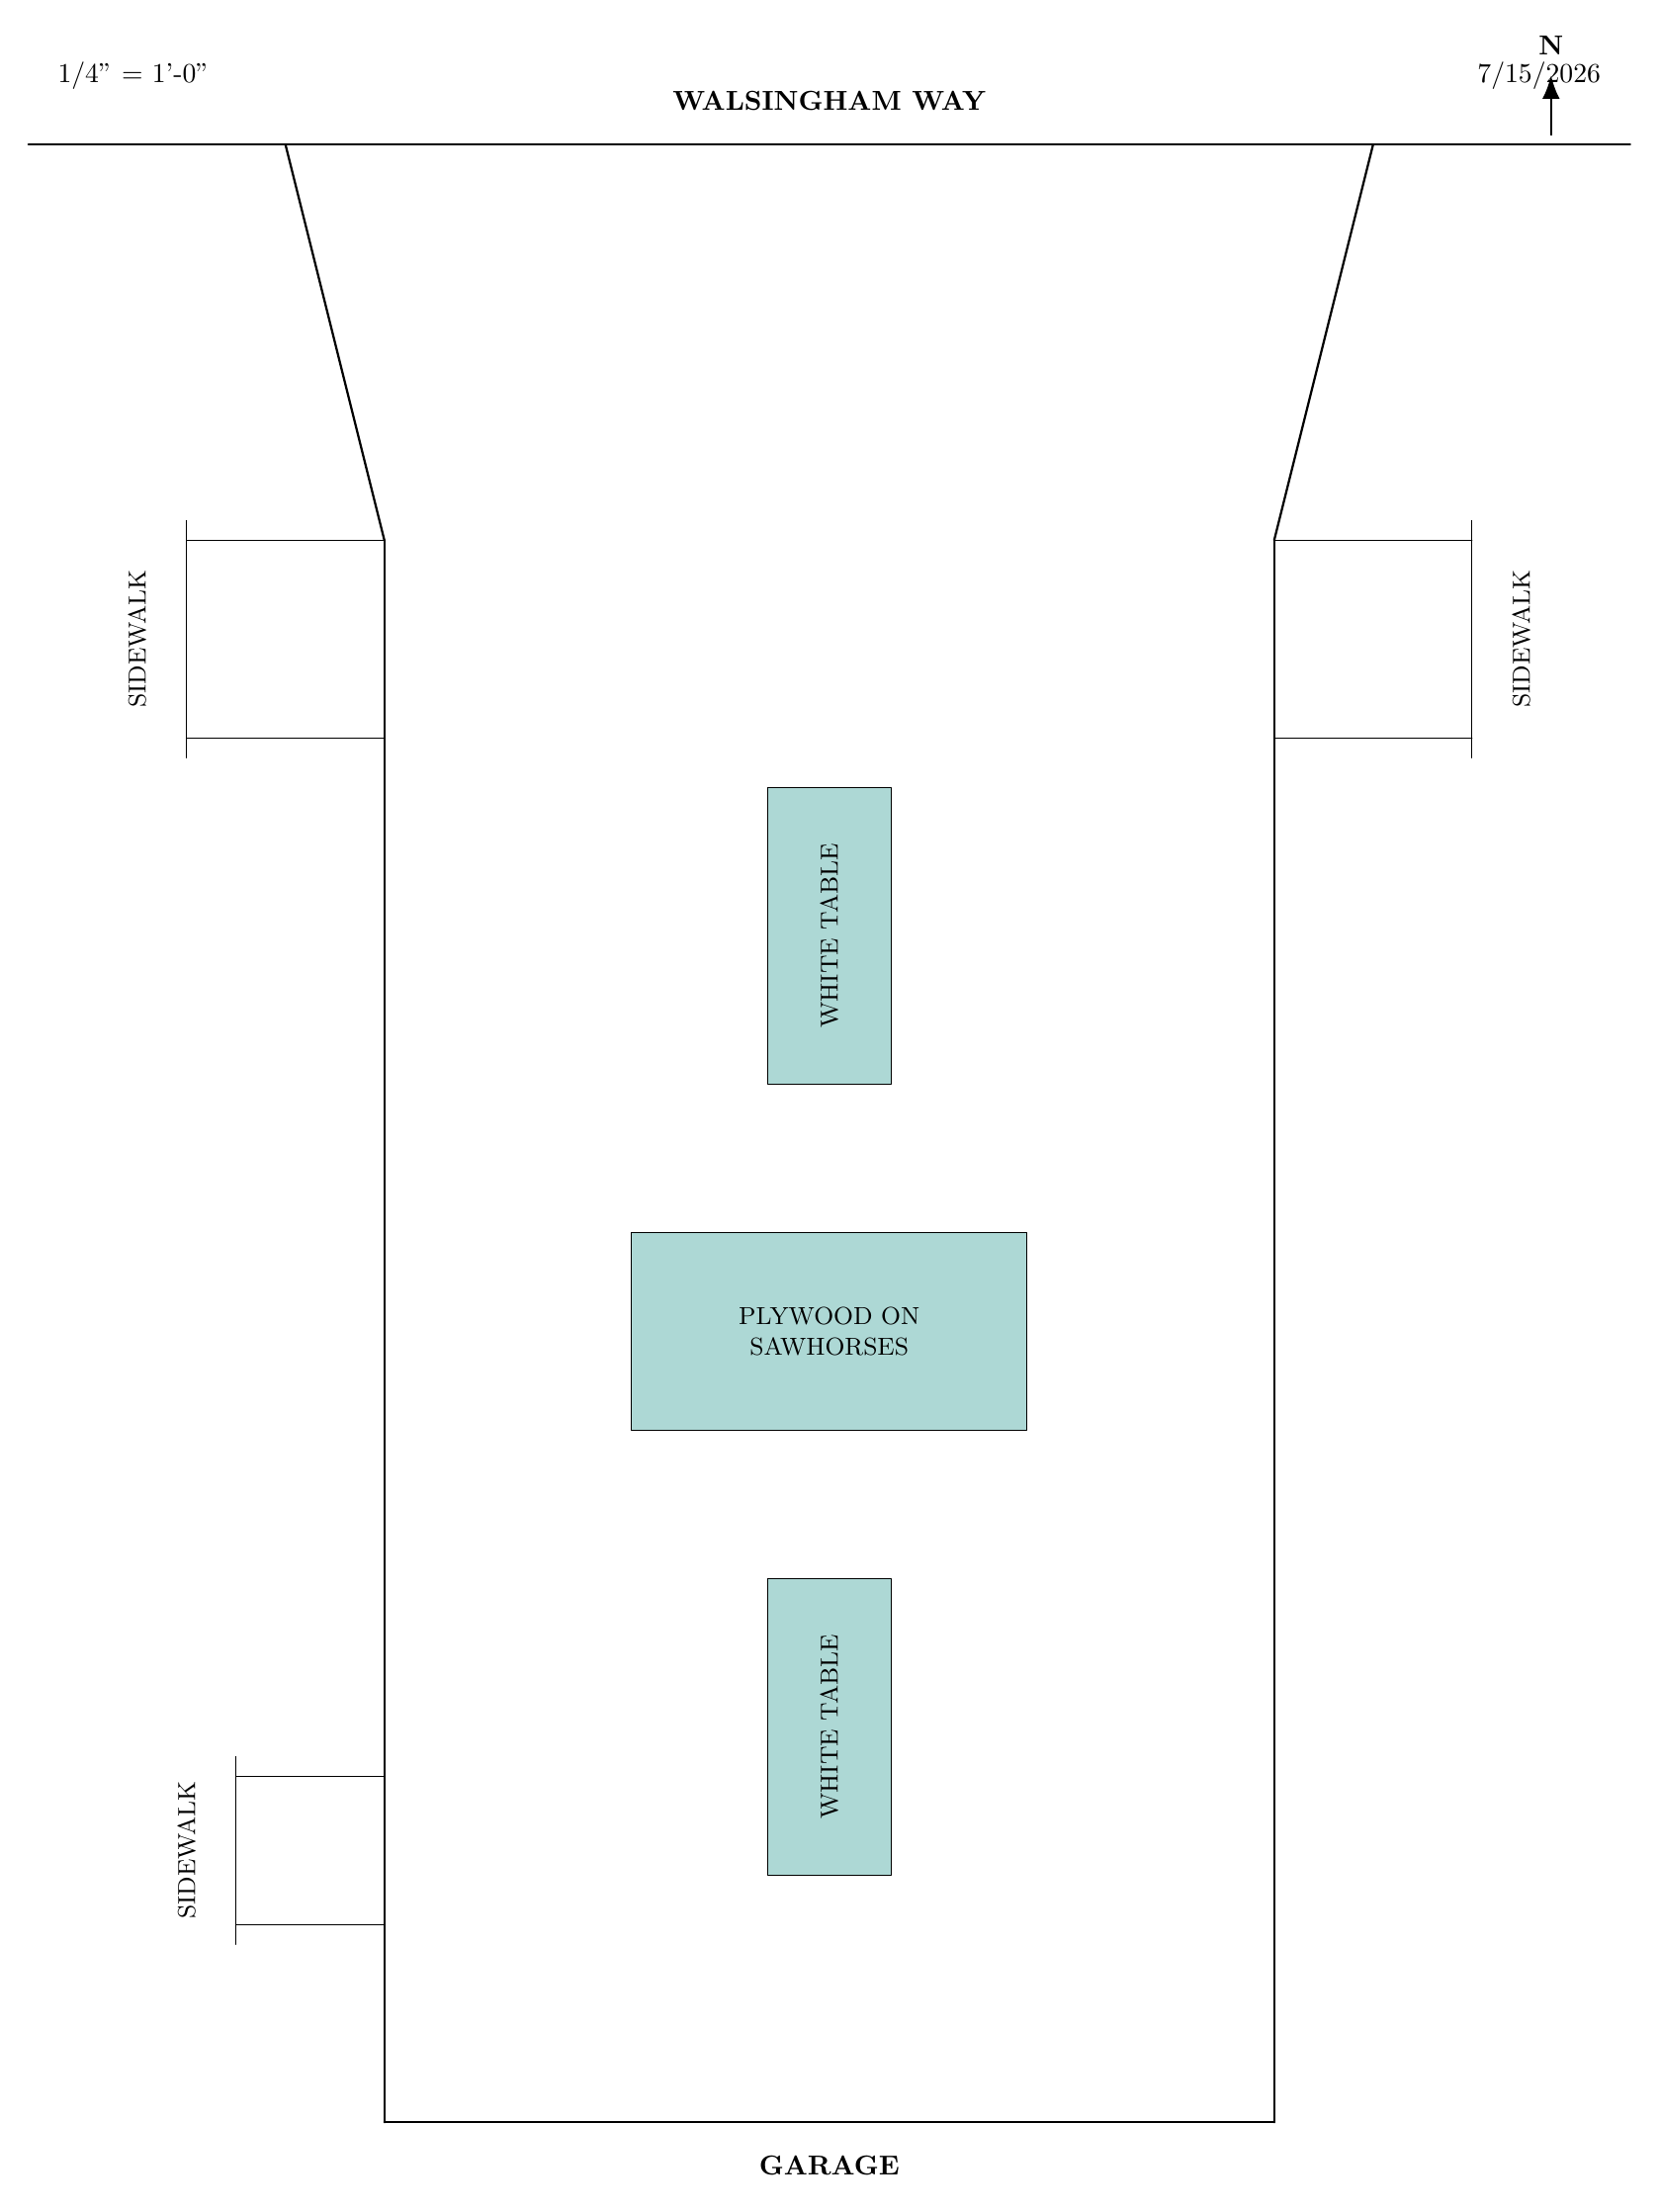
\begin{tikzpicture}[x=1in,y=1in,line join=round,line cap=round]

  % ---- reference values (page inches) ----
  % Horizontal
  \def\driveLx{2.0}      % left edge of driveway
  \def\driveRx{6.5}       % right edge of driveway
  \def\driveCx{4.25}      % driveway centerline
  \def\sideMainW{1.0}     % width of the two sidewalks by the street
  \def\sideLowW{0.75}     % width of the lower-left sidewalk
  \def\flareOut{0.5}      % each flare kicks out this much beyond the driveway edge

  % Vertical (all measured up from the garage line)
  \def\garageY{0.4}
  \def\streetY{10.4}      % garage + 10in driveway length
  \def\sideMainY{7.4}     % 7in from garage
  \def\sideLowY{1.4}      % 1in from garage
  \def\tableNCy{6.4}      % north table centerline, 6in from garage
  \def\plywoodCy{4.4}     % plywood centerline, 4in from garage
  \def\tableScy{2.4}      % south table centerline, 2in from garage

  % Item sizes
  \def\tableW{0.625}      % 5/8in
  \def\tableH{1.5}
  \def\plyW{2.0}
  \def\plyH{1.0}

  % ---- street ----
  \draw[thick] (0.2,\streetY) -- (8.3,\streetY);
  \node[font=\bfseries] at (4.25,\streetY+0.22) {WALSINGHAM WAY};

  % ---- driveway verticals + flares ----
  \draw[thick] (\driveLx,\garageY) -- (\driveLx,\sideMainY+\sideMainW);
  \draw[thick] (\driveRx,\garageY) -- (\driveRx,\sideMainY+\sideMainW);
  \draw[thick] (\driveLx,\sideMainY+\sideMainW) -- ({\driveLx-\flareOut},\streetY);
  \draw[thick] (\driveRx,\sideMainY+\sideMainW) -- ({\driveRx+\flareOut},\streetY);

  % ---- garage line ----
  \draw[thick] (\driveLx,\garageY) -- (\driveRx,\garageY);
  \node[font=\bfseries] at (\driveCx,\garageY-0.22) {GARAGE};

  % ---- sidewalks (drawn as dimension-style brackets, per sketch) ----
  % left, main (near street)
  \draw (\driveLx-\sideMainW,\sideMainY) -- (\driveLx,\sideMainY);
  \draw (\driveLx-\sideMainW,\sideMainY+\sideMainW) -- (\driveLx,\sideMainY+\sideMainW);
  \draw (\driveLx-\sideMainW,\sideMainY-0.1) -- (\driveLx-\sideMainW,\sideMainY+\sideMainW+0.1);
  \node[rotate=90,font=\small] at (\driveLx-\sideMainW-0.25,\sideMainY+\sideMainW/2) {SIDEWALK};

  % right, main (near street)
  \draw (\driveRx,\sideMainY) -- (\driveRx+\sideMainW,\sideMainY);
  \draw (\driveRx,\sideMainY+\sideMainW) -- (\driveRx+\sideMainW,\sideMainY+\sideMainW);
  \draw (\driveRx+\sideMainW,\sideMainY-0.1) -- (\driveRx+\sideMainW,\sideMainY+\sideMainW+0.1);
  \node[rotate=90,font=\small] at (\driveRx+\sideMainW+0.25,\sideMainY+\sideMainW/2) {SIDEWALK};

  % lower left sidewalk (left side only)
  \draw (\driveLx-\sideLowW,\sideLowY) -- (\driveLx,\sideLowY);
  \draw (\driveLx-\sideLowW,\sideLowY+\sideLowW) -- (\driveLx,\sideLowY+\sideLowW);
  \draw (\driveLx-\sideLowW,\sideLowY-0.1) -- (\driveLx-\sideLowW,\sideLowY+\sideLowW+0.1);
  \node[rotate=90,font=\small] at (\driveLx-\sideLowW-0.25,\sideLowY+\sideLowW/2) {SIDEWALK};

  % ---- items on the driveway ----
  \definecolor{noteteal}{RGB}{173,216,213}

  % north white table
  \draw[fill=noteteal] ({\driveCx-\tableW/2},{\tableNCy-\tableH/2}) rectangle ({\driveCx+\tableW/2},{\tableNCy+\tableH/2});
  \node[rotate=90,font=\small] at (\driveCx,\tableNCy) {WHITE TABLE};

  % plywood on sawhorses
  \draw[fill=noteteal] ({\driveCx-\plyW/2},{\plywoodCy-\plyH/2}) rectangle ({\driveCx+\plyW/2},{\plywoodCy+\plyH/2});
  \node[font=\small,align=center] at (\driveCx,\plywoodCy) {PLYWOOD ON\\SAWHORSES};

  % south white table
  \draw[fill=noteteal] ({\driveCx-\tableW/2},{\tableScy-\tableH/2}) rectangle ({\driveCx+\tableW/2},{\tableScy+\tableH/2});
  \node[rotate=90,font=\small] at (\driveCx,\tableScy) {WHITE TABLE};

  % ---- title block: scale + date ----
  \node[anchor=west] at (0.3,10.75) {1/4" = 1'-0"};
  \node[anchor=east] at (8.2,10.75) {7/15/2026};

  % ---- north arrow ----
  \draw[thick,-{Latex[length=3mm]}] (7.9,10.45) -- (7.9,10.75);
  \node[font=\bfseries] at (7.9,10.9) {N};

\end{tikzpicture}
\end{document}
